\documentclass[10pt]{article}

\usepackage[utf8]{inputenc}
\usepackage[IL2]{fontenc}
\usepackage{mathptmx}
\usepackage[a4paper, margin=1cm, noheadfoot]{geometry}
\usepackage[czech]{babel}
\usepackage[pdftex, unicode, hidelinks]{hyperref}
\usepackage[final]{pdfpages}
\usepackage{enumitem}

\hypersetup {
    pdfauthor={Ondřej Ondryáš (xondry02)},
    pdftitle={Návrh číslicových systémů: výstupní zpráva k projektu „Přístupový terminál“}
}

\title{Návrh číslicových systémů: výstupní zpráva}
\author{Ondřej Ondryáš (xondry02)}
\date{\today}

\begin{document}
\thispagestyle{empty}
\centering
{\large\bfseries Návrh číslicových systémů: výstupní zpráva k projektu „Přístupový terminál“}
\renewcommand{\labelitemi}{\textendash}
\begin{description}[itemsep=-1mm]
    \item[Jméno:] Ondřej Ondryáš
    \item[Login:] xondry02
    \item[Přístupové kódy:] 2051695357; 2093644584
    \item[Vstupní signály:]
        \begin{itemize}[leftmargin=0cm, itemindent=0.15cm]
            \item[]
            \item \texttt{KEY(15:0)} -- v diagramu označeno \texttt{K}. Symbol \# odpovídá hodnotě \textbf{15}. Zápis \texttt{K<>X,Y} znamená $KEY(X)=0$ AND $KEY(Y)=0$.
            \item \texttt{CNT\_OF} -- v diagramu označeno \texttt{COF}. Pokud není u přechodu uveden, předpokládá se hodnota \textbf{0}.
        \end{itemize}
    \item[Výstupní signály:]
        \begin{description}[leftmargin=0cm, itemindent=-0.1cm]
            \item[]
            \item[Moorovy výstupy:] \texttt{FSM\_CNT\_CE, FSM\_MX\_MEM, FSM\_MX\_LCD}
            \item[Mealyho výstupy:] \texttt{FSM\_LCD\_WR, FSM\_LCD\_CLR}
        \end{description}
\end{description}

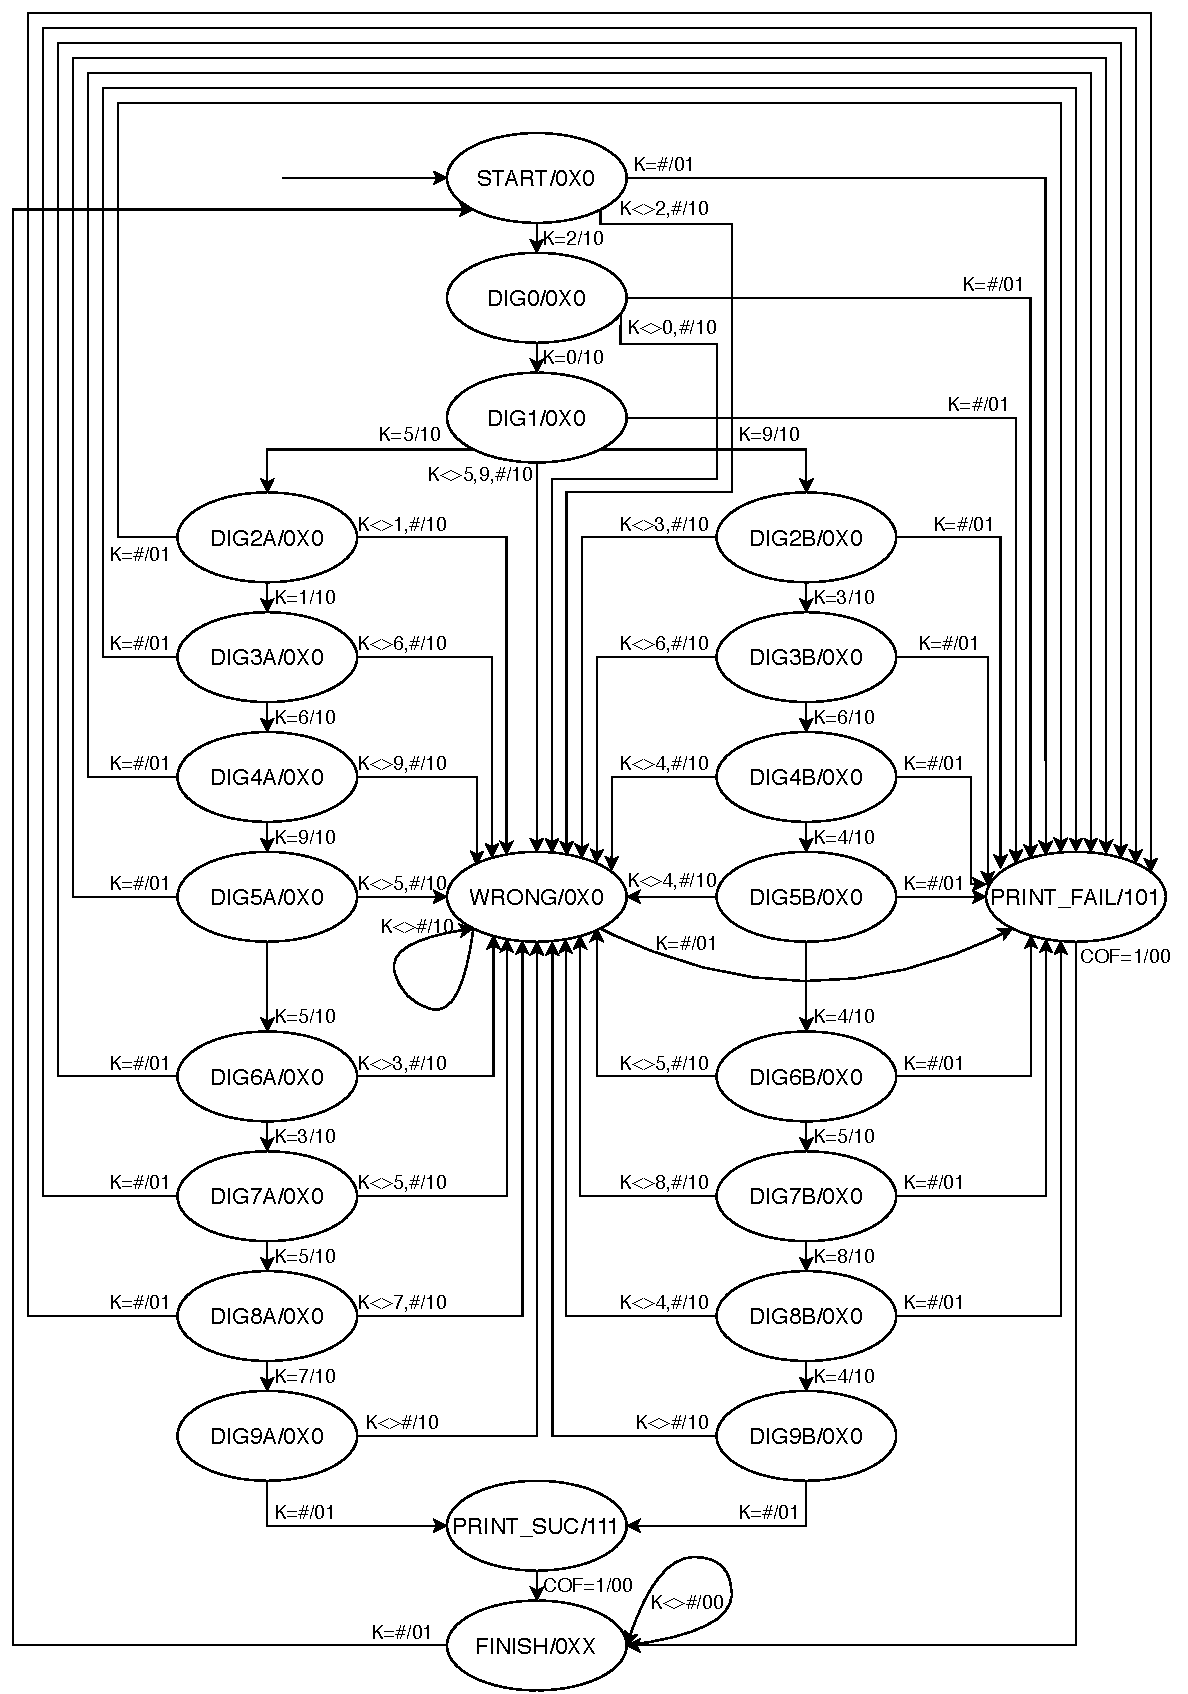
\includegraphics[height=0.825\textheight]{dia.pdf}

\end{document}
